\documentclass[11pt]{article}
\usepackage[T1]{fontenc}
\usepackage[utf8]{inputenc}
\usepackage{lmodern,microtype}
\usepackage[margin=0.93in,headheight=15pt]{geometry}
\usepackage{amsmath,amssymb,amsthm,mathtools}
\usepackage{booktabs,longtable,array,tabularx}
\usepackage{enumitem,xcolor,xurl,hyperref,fancyhdr,listings}
\usepackage{tikz,placeins}
\usetikzlibrary{arrows.meta,positioning,fit}
\definecolor{ink}{RGB}{28,56,79}
\hypersetup{colorlinks=true,linkcolor=ink,citecolor=ink,urlcolor=ink,
 pdftitle={Optimal Deferred-Handle Kernels via Ordered Incidence Interfaces},
 pdfauthor={ProveIt research continuation developed with ChatGPT}}
\pagestyle{fancy}\fancyhf{}
\fancyhead[L]{\small Ordered incidence interfaces}
\fancyhead[R]{\small ProveIt research continuation}
\fancyfoot[C]{\thepage}
\setlength{\parskip}{4pt}\setlength{\parindent}{1.2em}
\setlength{\emergencystretch}{2em}
\setlist{itemsep=3pt,topsep=5pt}
\lstset{basicstyle=\small\ttfamily,columns=fullflexible,breaklines=true,
 frame=single,framesep=5pt,showstringspaces=false}
\newtheorem{theorem}{Theorem}[section]
\newtheorem{lemma}[theorem]{Lemma}
\newtheorem{proposition}[theorem]{Proposition}
\newtheorem{corollary}[theorem]{Corollary}
\theoremstyle{definition}\newtheorem{definition}[theorem]{Definition}
\newtheorem{example}[theorem]{Example}
\theoremstyle{remark}\newtheorem{remark}[theorem]{Remark}
\newcommand{\N}{\mathbb N}
\newcommand{\sat}{\operatorname{sat}}
\newcommand{\supp}{\operatorname{supp}}
\newcommand{\tw}{\operatorname{tw}}
\newcommand{\poly}{\operatorname{poly}}
\newcommand{\Reach}{\operatorname{Reach}}
\newcommand{\code}[1]{\texttt{\detokenize{#1}}}
\newcommand{\pin}{\texttt{c6d0ec8aa0b6308310ab6c081ba29d8bc363ede5}}
% Inlined results/summary_macros.tex
% Generated from the recorded audit and benchmark, not estimates.
\newcommand{\NewTests}{47}
\newcommand{\ExhaustiveCases}{21,735}
\newcommand{\ChainOld}{750.321}
\newcommand{\ChainFactored}{733.550}
\newcommand{\ChainNew}{6.555}
\newcommand{\ChainRatio}{111.91}
\newcommand{\FanRatio}{135.46}


\begin{document}
\begin{titlepage}
\centering
\vspace*{0.3in}
{\LARGE\bfseries Optimal Deferred-Handle Kernels\\[5pt]
via Ordered Incidence Interfaces\par}
\vspace{0.22in}
{\large Exact $2^{O(t\log t)}$ optimization,\\[3pt]
linear two-incidence certificates, and a connected separation family\par}
\vspace{0.3in}
{Research continuation for Vladimir Reshetnikov's ProveIt project\\
Developed with ChatGPT\\[5pt]12 October 2026\par}
\vspace{0.25in}
\begin{minipage}{0.94\textwidth}
\begin{abstract}
The current geometric-core implementation already decides full positive singleton cancellation by a sparse column queue. The next optimization is different: minimize the handles that must remain when full cancellation is impossible. The immediate predecessor solves this by enumerating deferred row subsets and asks whether incidence decompositions improve the search.

We prove that, given a width-$t$ tree decomposition of the pivot-capable column incidence graph, minimum-weight deferral is computable in
\[
 (\lambda+q)^{O(1)}2^{O(t\log(t+2))},
\]
where $\lambda$ is the binary input length and $q$ is the decomposition size. No bound on the number of deferred rows is needed. The essential representation is an active boundary order with one processed-pivot bit per active vertex. Compatible topological orders amalgamate across separators, so an alternating-path reachability matrix is unnecessary. A bag of size $b$ has fewer than $e^{1/2}2^b b!$ states.

A second theorem gives exact weighted optimization by directed reachability and source strongly connected components when each pivot-capable column meets at most two rows. Its optimum has an independent linear-incidence lower-bound certificate. A connected family with $3q$ rows has width three and minimum deferral $q+1$, separating the new parameter regime from small-deferral enumeration.

The package contains a standard-library implementation, independent certificate replay, \NewTests\ unit tests, \ExhaustiveCases\ exhaustive matrix cases, weighted and alternate-decomposition audits, and paired completed-query measurements against actual predecessor code. It improves a specified local optimization problem. Ordered geometric transport, admissible hierarchy construction, and global restart bounds remain separate obligations; an unrestricted quasi-polynomial unknot recognizer is not claimed.
\end{abstract}
\end{minipage}
\vfill
{\small Targeted source revision: \pin\par}
{\small Proofs and finite audits are complementary; this is not a proof-assistant formalization.\par}
\end{titlepage}

\tableofcontents
\newpage

\section{Research position and the precise advance}
\label{sec:position}

\subsection{The checkpoint actually inspected}
The maintained \code{core_handlebody.py} now contains \code{column_cancellation_plan}. It retains the older minimum-fill producer as a comparison routine and uses the column queue when the first leaf pass stalls. Thus it would be incorrect to present sparse full-row cancellation as new implementation work here. The independently maintained verifier reconstructs unsigned occurrences from the attaching cycles and does not accept an arbitrary numerical summary as source authentication \cite{core,verify}.

The maintained parallelity synthesis is also ahead of an older top-level description: it constructs the all-dimensional source parallelity bundle and proves an inherited complementary core with at most $30T$ handles for $T$ source tetrahedra. Its bounded core is not automatically an admissible patterned handle structure \cite{parallelity}. The present work uses neither a presumed missing core bound nor presumed automatic admissibility as its research premise.

Our immediate predecessor, \emph{Rectangular Cancellation Without Search}, proves the exact positive-cancellation criterion and minimum-deferral characterization. Its complete optimization enumerates subsets in increasing cardinality, with cost proportional to
\begin{equation}
 \sum_{j=0}^{k}\binom mj
 \label{eq:old}
\end{equation}
when the optimum is at most $k$. Its further-research question 7 explicitly proposes exploiting an incidence-graph decomposition \cite{positive}. We resolve that question for supplied tree decompositions, including binary row weights, unit-eligibility restrictions, independent feasibility replay, and a useful special case with independently certifiable optimality.

\subsection{The theorem, informally}
Rows are two-handles and columns are one-handle cocores only when an enclosing geometric construction authenticates that interpretation. Numerically, a pivot removes a unit entry's row and column and positively substitutes its other occurrences into the remaining rows. A \emph{deferred} row is never pivoted. It remains a genuine part of the kernel and receives the passive updates.

The new parameter is the width of the incidence interface, not the size of the residual kernel. We first discard, for decision purposes only, columns containing no unit. All other nonzero entries of every retained column remain in the incidence graph, including entries greater than one. Given a tree decomposition of this graph with bags of size at most $t+1$, the optimum can be computed with a factorial, rather than quadratic-exponential, interface state space. The exact theorem is Theorem~\ref{thm:main}.

This is a substantive change of regime. The connected family in Theorem~\ref{thm:chain} has unbounded optimal deferral but a fixed width-three decomposition. The predecessor's increasing-subset algorithm necessarily examines exponentially many subsets on that family. The new dynamic program takes polynomial encoded time, and linear-many fixed-width transitions when the displayed decomposition is supplied.

\subsection{Attribution and the literature boundary}
Uniquely restricted matchings and their matrix-triangularization interpretation are classical. The maximum problem is NP-hard already on bipartite graphs \cite{golumbic}. Chaudhary, Sau and Zehavi's 2025 paper gives a deterministic general-graph treewidth algorithm with stated time $O(2^{\tw^2/2}|V|)$ \cite{csz}. Our theorem specializes to bipartite incidence graphs with unit-eligible pivots and row costs, and gives $2^{O(t\log t)}$ dependence on a supplied width. It is not a claim about arbitrary non-bipartite graphs.

Topological ordering, tree-decomposition dynamic programming, strongly connected components, and weighted obstruction packings are not claimed inventions. The contribution is the closed order-state formulation for this cancellation optimization, its proved complexity, the two-incidence characterization, the connected separation family, and their executed implementation. The matching equivalence and the predecessor's stopping and passive-transport results are attributed below. A targeted literature search is not an exhaustive priority determination; in particular, we do not claim to have excluded every earlier bipartite formulation with the same asymptotic bound.

\subsection{Two primary announcement exponents should not be conflated}
There is a real source distinction. The February 2021 Oxford announcement and the linked February slides state $n^{O(\log n)}$ \cite{announcement,february}. The March Oxford handout states $2^{O((\log n)^3)}=n^{O((\log n)^2)}$ and displays that bound again after its hierarchy estimates \cite{march}. Thus neither expression should be described as the sole exponent appearing in the announcements. We distinguish both scales in Section~\ref{sec:global}.

The July 2026 manuscript's Section 9 bounds iteration counts by $L(g+1)^L$ while explicitly separating insufficiently specified operation costs \cite{lackenby}. We do not turn that count into a running-time theorem for the maintained recognizer. The present theorem concerns one exact local operation and can contribute to either quasi-polynomial target once the remaining geometric and global estimates are supplied.

\section{The positive calculus and the optimization objective}
\label{sec:calculus}

\subsection{Finite data, saturation and original row identities}
Let $R$ and $C$ be finite sets, and let
\[
 A=(a_{rc})\in\N^{R\times C},\qquad m=|R|.
\]
The input explicitly stores its nonzero entries, including their binary values. Empty rows are retained. Completely zero columns may be omitted from this numerical optimization, but a native caller must keep them in its geometric handle inventory.

Write $\sat(x)=\min(2,x)$. A positive singleton pivot at $(r,c)$ requires $a_{rc}=1$, removes row $r$ and column $c$, and replaces every other entry by
\begin{equation}
 a'_{ih}=\sat(a_{ih}+a_{ic}a_{rh}).
 \label{eq:pivot}
\end{equation}
Unsaturated positive transport uses the same expression without $\sat$. There is no subtraction, free-group reduction, or signed exponent-sum cancellation in this calculus.

For nonnegative integers,
\[
 \sat(x+y)=\sat(\sat(x)+\sat(y)),\qquad
 \sat(xy)=\sat(\sat(x)\sat(y)).
\]
Consequently, retaining only zero, one and at-least-two is exact for deciding which pivots are legal throughout a positive schedule. Large source counts are not large expanded incidence lists.

A column is \emph{private} for an active row $r$ if its sum over the active rows is one. This entails $a_{rc}=1$ and zero entries in that column in every other active row. A private pivot creates no fill in the other active rows.

\subsection{The stopping obstruction, with a self-contained proof}
\begin{definition}
A nonempty row set $S\subseteq R$ is \emph{stopping} if, for every column $h$,
\[
 \sum_{i\in S}a_{ih}\ne1.
\]
Equivalently, every such sum is zero or at least two.
\end{definition}

The following proof restates the predecessor's exact obstruction argument so that the subsequent optimization does not rely on an unexplained matrix heuristic \cite{positive}.

\begin{lemma}[Stopping sets survive positive pivots]
\label{lem:stop}
After any legal positive pivot, a stopping set has a nonempty surviving subset that is stopping in the new matrix.
\end{lemma}
\begin{proof}
Use unsaturated entries temporarily; saturation does not change whether a nonnegative column sum is one. Pivot at $(r,c)$ and put $s_h=\sum_{i\in S}a_{ih}$.

If $r\notin S$, the new sum in column $h\ne c$ is $s_h+s_ca_{rh}$. Each $s_h$ and $s_c$ is zero or at least two, so the new sum cannot be one. The row set remains nonempty.

If $r\in S$, then $a_{rc}=1$ and stopping implies $s_c\ge2$. Thus $S'=S\setminus\{r\}$ is nonempty. Its new sum in column $h\ne c$ is
\[
 (s_h-a_{rh})+(s_c-1)a_{rh}
   =s_h+(s_c-2)a_{rh}.
\]
If $s_h\ge2$, this is at least two. If $s_h=0$, nonnegativity implies $a_{rh}=0$, so it is zero. Again it cannot be one. Applying saturation proves the assertion in the stated calculus.
\end{proof}

\begin{proposition}[Full cancellation criterion]
\label{prop:full}
The following conditions are equivalent: some positive singleton schedule removes every row; the matrix has no stopping set; private-column peeling removes every row.
\end{proposition}
\begin{proof}
A stopping set prevents complete removal by Lemma~\ref{lem:stop}. If private peeling stalls on nonempty rows, every surviving column has sum zero or at least two. Previously pivoted columns have zero entries in those rows, since each pivot was private. Hence the residual rows form a stopping set in the original matrix. The absence of a stopping set therefore forces peeling to finish. Finally private pivots are legal positive pivots.
\end{proof}

\subsection{Weighted deferral is exact partial cancellation}
Assign each row a nonnegative binary integer weight $w_r$. For $D\subseteq R$, write $w(D)=\sum_{r\in D}w_r$. Define
\begin{equation}
 \delta_w(A)=\min\{w(D): A[R\setminus D,C]\text{ admits full private peeling}\}.
 \label{eq:objective}
\end{equation}
Unit weights give $\delta(A)$. The all-deferred set is always feasible, including when there are no pivot-capable columns.

\begin{proposition}[Deferred-row equivalence]
\label{prop:defer}
Exactly the rows $R\setminus D$ can be removed by a positive schedule that never pivots a row of $D$ if and only if $D$ meets every stopping set of $A$. Equivalently, $A[R\setminus D,C]$ admits complete private peeling.
\end{proposition}
\begin{proof}
Restriction to the active rows commutes with every update using an active donor row: no passive entry appears in an active-row update. Thus a complete positive schedule on the active restriction is necessary, and Proposition~\ref{prop:full} replaces it by a private schedule. Conversely that private schedule is legal in the full matrix. Deferred entries may change, but cannot change active entries. A stopping set in the restriction is exactly an original stopping set disjoint from $D$.
\end{proof}

For unit weights, the longest positive schedule has $m-\delta(A)$ pivots. For general weights, $\delta_w$ minimizes the original weights of the retained row identities. It does \emph{not} automatically minimize transported word length, final crossing count, or the subsequent difficulty of resolving the residual geometry.

The implementation breaks equal-weight ties by minimizing $|D|$. It stores cost pairs $(w(D),|D|)$ lexicographically. This harmless secondary objective handles zero weights deterministically and does not change the theorem about minimum total weight.

\section{The pivot-capable incidence graph}
\label{sec:graph}

\subsection{Safe removal of uniformly nonunit columns}
Let
\[
 C_1=\{c\in C:\text{some }a_{rc}=1\}.
\]
A column outside $C_1$ has all entries zero or at least two.

\begin{proposition}[Decision-only omission]
\label{prop:omission}
Deleting $C\setminus C_1$ preserves every feasible deferred set and therefore every weighted optimum. The omitted columns must still be retained for passive transport and geometric census when those outputs are required.
\end{proposition}
\begin{proof}
An omitted column has sum zero or at least two on every row subset. It imposes no restriction on the stopping-set condition. Equivalently, positive additions and products of nonunit nonnegative entries cannot produce a unit in that column. Its entries never authorize a pivot. Proposition~\ref{prop:defer} applies to each row restriction.
\end{proof}

This is a deferral-compatible use of the predecessor's uniform-nonunit omission principle \cite{positive}. It is not permissible to omit a column merely because its \emph{total} is at least two. For example, two different entries equal to one can become private after one of their rows disappears.

\begin{definition}[Decision incidence graph]
The graph $G_1(A)$ is bipartite with vertices $R\sqcup C_1$. It has an edge $rc$ exactly when $a_{rc}>0$. The edge is \emph{eligible} exactly when $a_{rc}=1$.
\end{definition}

All rows occur, including isolated rows. Nonunit edges in a pivot-capable column are essential blockers and are retained. In particular $G_1$ is not the graph of unit entries alone.

\subsection{Unit-eligible uniquely restricted matchings}
Choose active rows $U$ and a set $Z\subseteq C_1$ of pivot columns. Suppose a matching $M$ bijects $U$ to $Z$ using eligible edges. On the induced graph $G_1[U\sqcup Z]$, orient
\begin{equation}
 c\longrightarrow r\quad\text{for }rc\in M,
 \qquad
 r\longrightarrow c\quad\text{for }rc\notin M.
 \label{eq:orientation}
\end{equation}
Call the resulting digraph $\mathcal D_M$.

\begin{theorem}[Acyclic orientation characterization]
\label{thm:orientation}
For a row set $U$, the following are equivalent.
\begin{enumerate}[label=(\roman*)]
\item $A[U,C]$ has a complete private-column schedule.
\item There is an eligible matching saturating $U$ whose digraph $\mathcal D_M$ is acyclic.
\item There is an eligible uniquely restricted matching saturating $U$.
\end{enumerate}
Consequently, weighted deferral is a row-weighted unit-eligible bipartite uniquely restricted matching optimization.
\end{theorem}
\begin{proof}
A private schedule chooses distinct pivot columns, giving a matching. If row $r_i$ is pivoted using $c_i$, every other active row incident to $c_i$ was removed earlier. A directed cycle in~\eqref{eq:orientation} would require a cyclic sequence of strict precedences among pivot times. Thus (i) implies (ii).

Conversely, take a topological ordering of $\mathcal D_M$ and process its row vertices in that order. For the pivot column $c$ of $r$, every other incident active row $s$ satisfies $s\to c\to r$. It has already been removed, so $c$ is private for $r$. Eligibility makes the pivot entry one. Distinct matching columns ensure no column is reused.

At a row vertex, the only incoming edge in~\eqref{eq:orientation} is its matching edge; at a column vertex, the only outgoing edge is its matching edge. Therefore directed cycles are exactly alternating cycles of the matching. A second perfect matching on the same saturated vertices differs from $M$ by a nonempty union of alternating cycles. Conversely an alternating cycle can be flipped to produce a second matching. Hence (ii) and (iii) are equivalent.
\end{proof}

The last equivalence is the classical uniquely restricted matching criterion \cite{golumbic}; its eligible-edge and weighted-row use here is explicit. Since ordinary bipartite instances arise by taking $A$ to be a zero--one matrix and all weights one, the general optimization inherits NP-hardness. The width hypothesis in our algorithm is doing real work.

\subsection{Componentwise additivity}
\begin{proposition}
\label{prop:additive}
Let $R_1,\ldots,R_h$ be the row sets of the connected components of $G_1(A)$. Then
\[
 \delta_w(A)=\sum_{i=1}^h\delta_{w|R_i}(A[R_i,C]).
\]
Isolated rows are components and must be deferred.
\end{proposition}
\begin{proof}
Every pivot-capable column has all of its incident rows in one component. Thus complete private schedules combine across components and restrict to them. Uniformly nonunit columns may connect the original numerical support across these components, but Proposition~\ref{prop:omission} shows that they cannot affect feasibility.
\end{proof}

Our benchmarks include a component-factorized version of the actual predecessor enumeration. This avoids attributing an exponential advantage to a new algorithm when elementary component splitting already removes it.


\subsection{Optimize only the canonical stopping core}
\begin{proposition}[Safe full-matrix prepeeling]
\label{prop:prepeel}
Let $K\subseteq R$ be the residual row set after exhaustive private-column peeling on the full original matrix. For nonnegative original row weights,
\[
 \delta_w(A)=\delta_{w|K}(A[K,C]).
\]
There is an optimal deferred set contained in $K$. A private prefix producing $K$, followed by a feasible private schedule on the active restriction of $K$, gives a feasible schedule on the original active rows. The same assertion holds when ties in total weight are broken by the number of deferred rows.
\end{proposition}
\begin{proof}
Every original stopping set is contained in $K$. Indeed, at any stage at which all its rows remain, no private column can select one of those rows: such a column would have total one on that stopping set. Induction shows that no member of any stopping set is peeled. Conversely, a stopping subset of $K$ is stopping in the original matrix, because its definition only sums the rows of that subset.

By Proposition~\ref{prop:defer}, feasibility means meeting all stopping sets. Intersecting any feasible deferred set with $K$ therefore remains feasible and cannot increase a nonnegative weight sum or its cardinality. This proves equality of optima. Every prefix pivot column is zero on all then-surviving rows, so the prefix creates no fill on $K$ and leaves its original entries unchanged. If some members of $K$ are deferred, each prefix pivot remains private among the other active rows. Concatenating the residual private schedule proves the scheduling assertion.
\end{proof}

This is an optimization consequence of the predecessor's canonical stopping-core theory, not a new claim that the full-row decision needs treewidth machinery. In particular, an all-peeled input should return immediately. When a proper nonempty core remains, automatic mode optimizes its restriction and reconstructs a plan on the original row labels. A decomposition supplied by the caller is not silently reindexed; automatic core reduction is used only when the optimizer is constructing its own decomposition. In that case, the output records \code{decomposition_scope_rows} explicitly.

Applying the main algorithm to this restriction yields a bound in the width of $G_1(A[K,C])$, which can be smaller than the width of the unreduced incidence graph. All geometric and passive-count data outside the decision graph still remain in the original source inventory.

\section{Ordered separators replace reachability matrices}
\label{sec:amalgamation}

The main algorithmic point is that an interface need not remember every alternating path through the interior. It may instead guess a common linear extension of all the precedence constraints. The number of linear orders is factorial, which is asymptotically smaller than enumerating arbitrary binary relations on a boundary.

\begin{lemma}[Ordered-interface amalgamation]
\label{lem:amalgamation}
Let $D_1,D_2$ be finite acyclic digraphs. Their vertex sets intersect in $B$, and there are no edges between $V(D_1)\setminus B$ and $V(D_2)\setminus B$. Suppose $D_i$ has a topological order whose restriction to $B$ is the same order
\[
 b_1<b_2<\cdots<b_s.
\]
Then $D_1\cup D_2$ is acyclic and has a topological order with this same restriction.
\end{lemma}
\begin{proof}
Take witnessing topological orders. Each has the form
\[
 L_{i,0},b_1,L_{i,1},b_2,\ldots,b_s,L_{i,s},
\]
where the $L_{i,j}$ are possibly empty sequences of private vertices. Form
\[
 L_{1,0},L_{2,0},b_1,L_{1,1},L_{2,1},b_2,
 \ldots,b_s,L_{1,s},L_{2,s}.
\]
Its restriction to either vertex set is the original witnessing order. Every edge belongs to one of the two digraphs, so every edge points forward. This is the required topological order.
\end{proof}

\begin{corollary}[Exact separator summary]
\label{cor:summary}
For a fixed active boundary and fixed processed-matching flags, it is sufficient to store, for each boundary order, only the least-cost partial solution admitting that order. Discarding more expensive partial solutions with the same state cannot destroy a better global completion.
\end{corollary}
\begin{proof}
A completion attaches only through the bag. Any valid completed solution has a global topological order, whose restriction selects a stored boundary order. Replacing its partial interior by a cheaper solution with that order preserves matching compatibility through the identical flags. Lemma~\ref{lem:amalgamation} preserves acyclicity. Costs outside the bag add independently.
\end{proof}

\begin{example}[Why the order cannot be discarded]
One partial digraph may contain a path from a boundary vertex $u$ to a boundary vertex $v$, while another contains a path from $v$ to $u$. Each part is acyclic, but their union is not. The two parts admit no common boundary order. A join that remembered only the active vertices and matching flags could incorrectly accept their union. The delivered tests include a $K_{2,2}$ matching-cycle instance split across two children, precisely to expose this failure mode.
\end{example}

The lemma asserts existence of an order, not uniqueness of the interior or of its topological sorting. It does not claim that two equal order states are geometrically equivalent handle structures. Their interchangeability is only for this finite matching-and-deferral objective.

\section{Exact dynamic programming on a supplied decomposition}
\label{sec:dp}

\subsection{Decomposition contract and event assignment}
A tree decomposition of $G_1$ is a finite tree with bags $B_x\subseteq V(G_1)$ such that every vertex occurs in a bag, every edge has both endpoints in a bag, and the bags containing a fixed vertex form a connected subtree. Its width is $\max_x|B_x|-1$.

Root the tree. Assign each graph edge to exactly one bag containing its endpoints, for example the highest such bag. The intersection of the occurrence subtrees of its endpoints is connected, so the highest bag is well-defined. Process an assigned edge only at its owner. This prevents a matching incidence from being counted twice at a join.

One may use a standard introduce-vertex, introduce-edge, forget-vertex and join event tree. Our implementation accepts an ordinary bag tree directly. To bring a child bag to its parent bag, it first forgets child-only vertices and then introduces parent-only vertices. All resulting bags have size at most the larger of the two original bags. Multiple children are joined sequentially; edges owned by the parent are introduced afterward. The root is finally transformed to an empty bag. This realizes $O((t+1)q+s_1)$ elementary events, where $q$ is the number of supplied bags and $s_1=|E(G_1)|$.

\subsection{State semantics}
At a bag $B$, choose its active subset $S\subseteq B$. A row is active when it is to be eliminated; a column is active when it is selected as a pivot column. An inactive row is deferred, whereas an inactive column is simply not selected as a pivot.

The state is
\begin{equation}
 (\pi,\mu),
 \qquad
 \pi\text{ a linear order of }S,
 \quad \mu:S\longrightarrow\{0,1\}.
 \label{eq:state}
\end{equation}
The active subset is recoverable from the ordered list $\pi$. The bit $\mu(v)$ says whether the unique matching edge incident to $v$ has already been introduced in the processed part.

A partial realization of this state consists of the following finite choices. Some processed vertices are active. The introduced eligible matching edges form a matching on these vertices; each active vertex outside the bag has exactly one such edge, and each active bag vertex has exactly $\mu(v)$ such edges. Every introduced edge with active endpoints is oriented by~\eqref{eq:orientation}. This partial digraph is acyclic and has a topological order restricting to $\pi$ on the bag. The value stored for the state is the minimum total weight of inactive \emph{row vertices outside the bag}. Inactive bag rows have not yet been charged.

The latter convention is essential at joins. Otherwise the weight of a deferred boundary row could be counted independently in both child subtrees.

\subsection{Introduce a vertex}
Suppose $v$ enters the bag and has no introduced edge yet. There is an inactive choice, which leaves the order and flags unchanged. There is also an active choice for every insertion position of $v$ into $\pi$, with $\mu(v)=0$.

For soundness, take an existing witnessing topological order. The new vertex is isolated in the processed digraph and can be inserted so that the desired order on the bag results. Completeness follows by restricting a witnessing order of any enlarged partial solution. No row cost is charged at introduction.

\subsection{Introduce an incidence edge}
Suppose $rc$ is introduced, with $r\in R$ and $c\in C_1$.

If one endpoint is inactive, the edge is absent from the selected induced digraph and nothing changes. If both are active, their order determines the edge type:
\begin{equation}
\begin{array}{c|c|c}
\text{Boundary order}&\text{Required role}&\text{Condition}\\ \hline
r<_{\pi}c & \text{nonmatching edge }r\to c & \text{no flag change}\\
c<_{\pi}r & \text{matching edge }c\to r & a_{rc}=1,\ \mu(r)=\mu(c)=0.
\end{array}
\label{eq:edgeevent}
\end{equation}
In the second case set both flags to one. If its condition fails, discard the state.

Every accepted edge points forward in the witnessing topological order, so acyclicity is preserved. Conversely a partial realization's topological order forces exactly the indicated role for an introduced edge with active endpoints. Notice in particular that an entry greater than one cannot be reinterpreted as a matching edge merely to satisfy a convenient order.

\subsection{Forget a vertex}
If $v$ is active, it may be forgotten only when $\mu(v)=1$. Remove it from the order and flag map. If $v$ is inactive and a row, add $w_v$ to the stored cost. If it is an inactive column, add zero.

No edge incident to a forgotten vertex will be introduced later: all bags containing that vertex lie in the processed part once it leaves the boundary. Thus the matching condition is final at this point. Conversely, every valid partial realization with $v$ internal satisfies this condition. Restricting its topological order gives the new boundary order.

The tree-decomposition running-intersection property also ensures that each original row is forgotten above its occurrence subtree exactly once in the total computation. It may be introduced separately in different branches, but its cost is not separately paid there while it remains a boundary vertex.

\subsection{Join two children}
A pair of child states is compatible exactly when the two active ordered lists $\pi$ are identical and
\begin{equation}
 \mu_1(v)+\mu_2(v)\le1\quad(v\in S).
 \label{eq:join}
\end{equation}
The parent flags are their sum and the parent cost is the sum of child costs. Keep the smallest value for each resulting state.

The vertex sets private to the two subtrees are disjoint, and no original edge joins those private sets. The edge ownership rule makes the introduced edge sets disjoint. Condition~\eqref{eq:join} prevents a boundary vertex from being matched twice. Lemma~\ref{lem:amalgamation} supplies the common topological order, and the two cost sets are disjoint because neither child has charged its bag rows. This proves soundness.

For completeness, restrict any parent realization and one of its topological orders to the child vertex sets. Both restrictions induce the same bag order. Their flags satisfy~\eqref{eq:join}, their private row costs sum to the parent cost, and each is among the allowed child states. Keeping least-cost representatives cannot increase the optimum by Corollary~\ref{cor:summary}.

\subsection{The empty root and reconstruction}
At the empty root, every chosen active vertex has been matched exactly once and the complete chosen digraph is acyclic. Theorem~\ref{thm:orientation} converts it to a feasible deferred set. Conversely every feasible set has an eligible acyclic matching and a global topological order, and hence a consistent sequence of states. The root value is therefore the optimum.

The delivered implementation retains a small backpointer directed acyclic graph of forgotten deferred rows and joins. It does not export its chosen matching. Once the optimal deferred set is recovered, a separate private-column producer reconstructs a schedule on the original active restriction. An independent verifier then replays that schedule. Different optimal matching choices are allowed because the optimized objective concerns retained row identities, not a prescribed pivot order.

\begin{theorem}[Exact ordered-interface optimization]
\label{thm:main}
Let $A$ be a finite explicitly encoded nonnegative integer matrix with nonnegative binary row weights, and let $\mathcal T$ be a valid $q$-bag tree decomposition of $G_1(A)$ with width at most $t$. There is a deterministic algorithm computing $\delta_w(A)$ and an attaining deferred set with a private-column schedule in
\begin{equation}
 (\lambda+q)^{O(1)}2^{O(t\log(t+2))}
 \label{eq:mainbound}
\end{equation}
bit operations, where $\lambda$ includes matrix values, labels, weights and the encoded bag data. The same asymptotic form bounds space. The theorem requires no bound on $\delta(A)$, on $|D|$, or on the numerical magnitude of a matrix entry beyond its binary encoding length.
\end{theorem}
\begin{proof}
The preceding transition proofs establish soundness, completeness and exact minimization by induction on the event tree. The empty-root argument identifies the optimum, and independent private peeling reconstructs a schedule. The state and arithmetic bounds in the next section give~\eqref{eq:mainbound}. When the graph is empty the answer is immediate.
\end{proof}

\section{State count, bit complexity and implementation costs}
\label{sec:complexity}

\subsection{A factorial state bound}
For a bag of size $b$, choose $s$ active vertices, order them, and choose their $s$ flags. Thus
\begin{align}
 P_b
 &=\sum_{s=0}^b\binom bs s!2^s\notag\\
 &=2^b b!\sum_{j=0}^b\frac{1}{2^j j!}
 < e^{1/2}2^b b!.
 \label{eq:states}
\end{align}
For a fixed ordered active set of size $s$, a join considers at most $4^s$ pairs of flag assignments; only $3^s$ of them are disjoint. Indexing child states by their ordered active list avoids a factorial-squared join. A conservative bound for the directly implemented pair loop is
\begin{equation}
 J_b=\sum_{s=0}^b\binom bs s!4^s
 <e^{1/4}4^b b!.
 \label{eq:joincount}
\end{equation}
Introduce, forget and edge events require only polynomially many operations per state. With $b=t+1$, both $P_b$ and $J_b$ are $2^{O(t\log(t+2))}$. Even simple comparison-based indexing adds only polynomial factors in the state-description length. These bounds do not assume that every formally enumerated state is realizable; actual tables are often much smaller.

\subsection{Arithmetic is measured in bits}
Let $W$ bound the bit length of an input row weight. Every stored primary cost is at most $\sum_r w_r$, so it has at most $W+\lceil\log_2(m+1)\rceil+O(1)$ bits. The secondary cardinality cost has $O(\log(m+1))$ bits. Cost addition and comparison therefore have polynomial bit cost.

An entry of a decision matrix is used only to distinguish zero, one and greater than one. Reading and testing its binary value is charged to $\lambda$; its numerical magnitude is never iterated over. The implementation's stress tests include $16{,}385$-bit entries and weights.

The mathematical state representation may use bag-local flags. The prototype uses dense global vertex indices in Python integer masks for simplicity. Those masks can use $O(|V(G_1)|)$ bits rather than $O(t)$ bits. This affects polynomial factors, not~\eqref{eq:mainbound}, and is a clear implementation optimization opportunity rather than a hidden unit-cost assumption.

\subsection{Where the decomposition comes from}
The theorem takes a decomposition as input. The prototype validates the parent tree, vertex coverage, edge coverage and running intersection before using it. It also offers deterministic minimum-fill elimination to construct a valid decomposition. That heuristic does not certify minimum treewidth. An unlucky order may yield a much larger width than another valid decomposition.

For completeness, the elimination construction is simple. On eliminating $v$, record the bag consisting of $v$ and its remaining neighbors, and fill those neighbors to a clique. Attach this bag to the bag of its earliest-eliminated later neighbor, or to an empty super-root if there is no later neighbor. At the elimination of that parent neighbor, all the other recorded neighbors are still present and adjacent to it. Hence the child separator is contained in the parent bag, proving the running-intersection property. Original edges are covered at the earlier endpoint's elimination.

The straightforward heuristic repeatedly rescans candidates and can cost $O(N^4)$ elementary graph work in a conservative worst-case accounting, with $N=|V(G_1)|$. This is polynomial, but can dominate an otherwise narrow-width query. The large chain experiment supplies its explicit decomposition and charges construction and validation; the paired small-query benchmark charges heuristic construction.

\subsection{Practical caps are not negative decisions}
The public prototype defaults to a supplied-width cap of nine, a table cap of $250{,}000$ states, and a dynamic-program candidate-work cap of $20{,}000{,}000$. These are configurable engineering limits, not hypotheses inserted into the mathematical theorem. Exhaustion returns \code{RESOURCE_LIMIT}; it does not return infeasibility, knottedness, or non-handlebodyness. A caller's cancellation exception is propagated.

The dynamic-program work cap does not bound input parsing or the minimum-fill preprocessing. The command-line admission cap and the caller's external time and memory controls remain relevant. This package is a research implementation, not a hardened service for arbitrary hostile inputs.

\section{A linear-incidence two-support theorem}
\label{sec:scc}

We now assume each \emph{pivot-capable} column has at most two nonzero row entries. Uniformly nonunit columns are unrestricted and remain irrelevant to the optimization by Proposition~\ref{prop:omission}. This distinction is useful for boundary kernels carrying large nonunit bulk families.

\subsection{Directed dependencies}
Build a digraph $H$ on the rows as follows. A pivot-capable column supported on one row $r$ necessarily has a unit there; put $r$ in a root set $Q$. For a column supported on two different rows $r,s$, insert
\begin{equation}
 s\longrightarrow r\quad\text{if }a_{rc}=1,
 \qquad
 r\longrightarrow s\quad\text{if }a_{sc}=1.
 \label{eq:rowarcs}
\end{equation}
The other positive entry in a column may be any nonunit value. Parallel arcs can be merged. The direction means that once the source row is absent, the target can use this column as a private unit.

\begin{lemma}[Peeling is exactly reachability]
\label{lem:reach}
For every deferred set $D$, the union of $D$ with all rows removable by private peeling is
\[
 \Reach_H(Q\cup D).
\]
\end{lemma}
\begin{proof}
Consider a row removed by a private pivot. A supporting column of size one makes it a root. A supporting column of size two has its other row already deferred or removed, and the target unit gives the appropriate arc. Induction on the peeling order proves that every removed row is reachable.

For the reverse direction, remove undeferred root rows using their singleton columns and then use any breadth-first reachability order. Suppose a first-reached row $r$ is reached from an already absent row $s$ via a column supported on $r,s$. That column is still available: it could not have been used earlier to remove $s$ while $r$ was active, because it would not then have been private. No third row could have used it. It now has just the target unit in the active matrix, so it removes $r$. Distinct first-arrival choices therefore yield a legal private schedule. Deferred roots need no pivot, and exhausted or duplicate arcs are harmless.
\end{proof}

The column-availability argument is important. A bare reachability analogy without this argument would not justify converting a reachability tree into a cancellation sequence, since pivot columns are consumed.

\subsection{Exact weighted optimum}
Set
\[
 U_0=R\setminus\Reach_H(Q).
\]
Consider the strongly connected components of $H[U_0]$, and its condensation digraph. Call a component a \emph{source component} when no condensation edge enters it.

\begin{theorem}[Weighted source-component formula]
\label{thm:scc}
Let $S_1,\ldots,S_a$ be these source components. Under the two-support hypothesis,
\begin{equation}
 \delta_w(A)=\sum_{i=1}^a\min_{r\in S_i}w_r.
 \label{eq:sccopt}
\end{equation}
Choosing a minimum-weight row from each $S_i$ is optimal. With unit weights, the optimum is the number of source components. The graph construction, reachability, component computation and schedule extraction require $O(m+|C_1|+s_1)$ incidence operations, in addition to parsing and binary-weight arithmetic.
\end{theorem}
\begin{proof}
No arc can enter $U_0$ from a row reachable from $Q$, since its endpoint would then also be reachable. A source component of $H[U_0]$ therefore has no incoming arc from anywhere outside that component, and it contains no root. Lemma~\ref{lem:reach} implies that a successful deferred set must contain a row of each $S_i$. This gives the lower bound in~\eqref{eq:sccopt}.

Conversely every vertex of a finite acyclic condensation graph is reachable from some source. One chosen row reaches its entire strongly connected component and then all its descendant components. The chosen seeds, together with $Q$, therefore reach every row. Lemma~\ref{lem:reach} gives a full active peeling schedule. Taking cheapest seeds attains the lower bound.

The directed graph has at most two arcs per retained column. Reachability and an iterative strongly connected component algorithm visit vertices and arcs a bounded number of times. Minimum-weight selection uses one pass per component. Private scheduling is another linear-incidence pass.
\end{proof}

The Python implementation canonicalizes labels and several outputs by sorting. Consequently its literal running time includes sorting and dictionary costs, not only the linear incidence count. The theorem concerns the usual already-indexed adjacency representation; binary cost comparisons and additions are charged at their bit lengths.

\subsection{Independent weighted optimality certificates}
\begin{proposition}[Tight stopping-pack certificates]
\label{prop:packing}
Let $D$ be a feasible deferred set for any nonnegative matrix. Suppose $S_1,\ldots,S_a$ are pairwise disjoint nonempty stopping row sets and
\[
 w(D)=\sum_{i=1}^a\min_{r\in S_i}w_r.
\]
Then $D$ is optimal. Feasibility, disjointness, the stopping property and this equality can be verified with linear incidence work, plus binary arithmetic and label bookkeeping.
\end{proposition}
\begin{proof}
Every feasible deferred set meets each $S_i$ by Proposition~\ref{prop:defer}. The sets are disjoint and weights nonnegative, so its cost is at least the displayed sum. The supplied feasible set attains that bound.

To check the stopping property, scan the entries in each supplied row set, saturating the accumulating column totals at two. Reject any total equal to one. Since the row sets are disjoint, each original incidence is scanned at most once in this stage. The private schedule checker separately scans the active incidence data a bounded number of times.
\end{proof}

The source components in Theorem~\ref{thm:scc} are stopping sets. A singleton-unit column would make a root. A two-support column with a target unit in the component and its other row outside would give an incoming arc. Every other contribution has total zero or at least two on the component. Therefore the theorem's lower bound is exactly a certificate of Proposition~\ref{prop:packing}.

The delivered optimality checker deliberately verifies this weaker sufficient property directly from the original matrix. It neither imports the dynamic program nor reruns the SCC finder or its dependency-graph construction. This gives a genuinely separate arithmetic route to the optimality conclusion. It does not need to assert that the supplied sets are precisely all the producer's source components.

Tight disjoint packings need not exist for general matrices. Three unit rows sharing one column require two deferrals, but a disjoint nonempty stopping-set packing has weight at most one. Thus failure of this certificate checker does not refute a general dynamic-program optimum.

\section{A connected constant-width separation family}
\label{sec:separation}

A disconnected family is not sufficient to demonstrate the need for the new method: Proposition~\ref{prop:additive} could already solve it block by block. We therefore give a connected example with unbounded optimal deferral.

For $q\ge1$, let block $i$ have rows $a_i,b_i,c_i$ and internal columns $x_i,y_i,z_i$, with all nine internal entries equal to one. For $0\le i<q-1$, add a bridge column $h_i$ with unit entries in exactly $c_i$ and $a_{i+1}$. There are no other entries. Denote the resulting matrix by $K_q$.

\begin{figure}[ht]
\centering
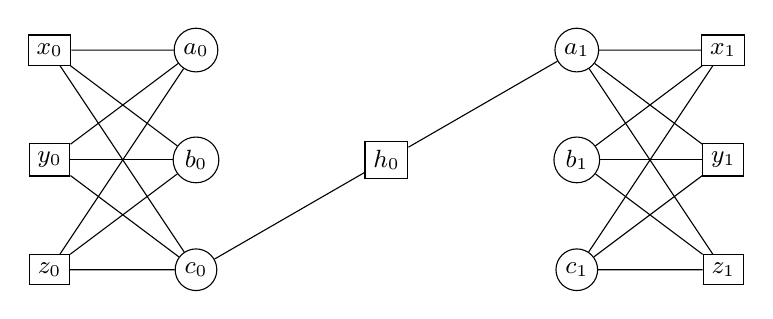
\begin{tikzpicture}[scale=0.93, every node/.style={font=\small},
 rv/.style={circle,draw,inner sep=2pt},cv/.style={rectangle,draw,inner sep=3pt}]
\foreach \name/\yy in {a/1.5,b/0,c/-1.5}{
 \node[rv] (\name0) at (0,\yy) {$\name_0$};
 \node[rv] (\name1) at (5.2,\yy) {$\name_1$};
}
\foreach \name/\yy in {x/1.5,y/0,z/-1.5}{
 \node[cv] (\name0) at (-2,\yy) {$\name_0$};
 \node[cv] (\name1) at (7.2,\yy) {$\name_1$};
}
\foreach \r in {a,b,c}{\foreach \c in {x,y,z}{
 \draw (\r0)--(\c0);\draw (\r1)--(\c1);
}}
\node[cv] (h) at (2.6,0) {$h_0$};
\draw (c0)--(h)--(a1);
\end{tikzpicture}
\caption{The incidence graph of $K_2$. Every drawn incidence is a unit. Each block is $K_{3,3}$ and the extra column bridges the two blocks. This is an explicit matrix family, not an asserted native normal-cut export.}
\label{fig:chain}
\end{figure}

\begin{theorem}[Connected width-three family]
\label{thm:chain}
The graph $G_1(K_q)$ is connected, has a width-three tree decomposition, and
\begin{equation}
 |R|=3q,\qquad |C|=4q-1,\qquad s=11q-2,\qquad
 \delta(K_q)=q+1.
 \label{eq:chain}
\end{equation}
The predecessor's increasing-cardinality subset algorithm must examine $2^{\Omega(q)}$ subsets before it can return an optimum. With the displayed decomposition, Theorem~\ref{thm:main} instead has polynomial encoded cost and $O(q)$ fixed-width events.
\end{theorem}
\begin{proof}
Connectivity and the counts follow from the construction. For a decomposition of one block, use three bags
\[
 \{a_i,b_i,c_i,x_i\},\quad
 \{a_i,b_i,c_i,y_i\},\quad
 \{a_i,b_i,c_i,z_i\},
\]
joined as a tree. For each bridge add the bag $\{c_i,h_i,a_{i+1}\}$ and connect it to one bag in each neighboring block. The resulting bag graph is a tree. Every row's occurrence bags are connected, every column occurs with all its endpoints, and the maximum bag size is four.

For the lower bound, consider a private schedule and its uniquely restricted matching. At most one internal column of any block can be a pivot column: two such matched columns and their two distinct matched rows would form an alternating four-cycle inside the all-unit block. The $q$ blocks therefore contribute at most $q$ internal pivots. There are only $q-1$ bridge columns, so there are at most $2q-1$ pivots in total. Proposition~\ref{prop:defer} gives $\delta(K_q)\ge3q-(2q-1)=q+1$.

For the upper bound, defer every $b_i$ and also $a_0$. Row $c_0$ is now the only active row of its block, so remove it using $x_0$. Then $h_0$ is private for $a_1$; remove $a_1$, and remove $c_1$ using $x_1$. Continue in this way. This removes $c_0,a_1,c_1,\ldots,a_{q-1},c_{q-1}$ and defers exactly $q+1$ rows.

Every subset of size at most $q$ fails. An increasing-size enumeration must therefore test at least $\binom{3q}{q}\ge 3^q$ subsets; the inequality follows from
\[
 \binom{3q}{q}=\prod_{j=0}^{q-1}\frac{3q-j}{q-j}\ge3^q.
\]
The decomposition has $4q-1$ bags of width three and the support size is linear in $q$. The stated contrast follows.
\end{proof}

The constant-width theorem is not an assertion that the synthetic benchmark is itself difficult for every possible algorithm. Its displayed construction has a direct optimum formula. It proves an unconditional separation between the predecessor's subset enumeration and the general ordered-interface method, and supplies a reproducible connected stress family rather than a claim about hard knots.

\subsection{Large deferral can also occur in actual ball presentations}
The predecessor realizes
\[
 H=\begin{pmatrix}1&1\\1&2\end{pmatrix}
\]
by two positive slides of a standard canceling two-handle disk system, without changing the underlying ball. Boundary-connected sums give matrices $\operatorname{diag}(H,\ldots,H)$ with $2q$ rows and deferral number $q$ \cite{positive}. Their decision graphs have width at most two. Thus even the geometric ball examples already distinguish small width from small deferral.

This uses the predecessor's geometric construction, not a new native source exporter. We do not assert that those handle presentations are outputs of the current normal-cut constructor. On the disconnected matrices, component-factored enumeration is already effective; the connected family $K_q$ avoids that particular explanation of the improvement.

\subsection{A connected two-support family}
For an additional directed-graph test, take the $q$ copies of $H$, add one row $z$, and for each block add a column having entry two in its first row and entry one in $z$. These new columns point toward $z$ in~\eqref{eq:rowarcs}. The graph is connected, its $q$ original block components are exactly the source strongly connected components, and $z$ is downstream. Theorem~\ref{thm:scc} gives optimum $q$ with unit weights. We call this the source-SCC fan in the benchmark.

The added rows and columns are numerical test data only; no ball or native normal-cut realization is claimed for this fan. Unlike the block-diagonal examples, elementary component factoring does not separate its decision graph.

\section{Witnesses, passive transport and geometric scope}
\label{sec:transport}

\subsection{Feasibility is checked independently of optimization}
A delivered plan contains a schema, deferred row identities, the cancellation pairs and the objective value. Given the source matrix, the verifier initializes column sums on the active rows and checks each pair $(r,c)$ by requiring that $r$ is still active, $c$ has not been consumed, and the active sum in $c$ is one with a unit at $(r,c)$. It deletes the row's original incidences from those sums and continues. Every active row must be removed exactly once, and the stated cost must equal the weight of the deferred set.

This checker uses neither a tree decomposition nor a dynamic-program order. It also does not accept the producer's optimum status as a proof of optimality. A valid private plan proves feasibility and cost. General optimality follows from the proved dynamic program or independent exhaustive checking on small cases. When a tight stopping packing is supplied, Proposition~\ref{prop:packing} additionally certifies optimality by direct input replay.

\subsection{Exact numerical transport is inherited, not reinvented}
Let the active private schedule be $(r_1,c_1),\ldots,(r_u,c_u)$. With these rows and pivot columns in this order, the unsaturated active matrix has the form
\[
 [I+Q\mid W],\qquad Q\text{ strictly upper triangular}.
\]
Write the passive rows as $[B\mid E]$. The predecessor's finite positive transport theorem gives
\begin{equation}
 E'=E+B(I-Q)^{-1}W
   =E+\sum_{j=0}^{u-1}BQ^jW.
 \label{eq:passive}
\end{equation}
The inverse is a finite geometric sum, not a signed Schur complement \cite{positive}.

To see why the formula applies, a passive coefficient in pivot column $c_i$ contributes its multiple of row $r_i$ to every later pivot and retained column. The active donor row is never altered by an earlier private pivot. Forward propagation therefore sums exactly the directed paths through the strictly upper triangular dependency matrix. The nilpotence $Q^u=0$ terminates the sum.

The package uses this attributed formula as a downstream consumer of the new optimal deferred set. It supports both exact and saturated numerical outputs. Its audit compares these outputs with the actual predecessor's transport implementation, rather than using equality of Euler characteristics as a surrogate.

\begin{proposition}[Polynomially encoded passive counts]
If original entries have at most $B_0$ bits and there are $n$ represented columns, each final passive entry after $u$ private active pivots has
\[
 O((u+1)(B_0+\log(n+1)))
\]
bits. Thus exact passive-count transport is polynomial in the explicit input length and output dimensions, even when passage counts are exponentially large.
\end{proposition}
\begin{proof}
For pivot row $r_i$, put $\sigma_i=\sum_{h\ne c_i}a_{r_i h}$. If a passive row has current total mass $M$ and coefficient $f$ in $c_i$, its new mass is $M-f+f\sigma_i$, at most $M\max(1,\sigma_i)$. Induction bounds the total mass by its initial mass times $\prod_i\max(1,\sigma_i)$. Both the initial mass and each $\sigma_i$ are at most $n2^{B_0}$. Taking binary logarithms proves the result, treating zero masses separately. This is the predecessor's mass argument applied after the new optimization \cite{positive}.
\end{proof}

\subsection{A complete worked weighted example}
Take
\[
 A=\begin{pmatrix}1&1\\1&2\end{pmatrix},\qquad
 (w_0,w_1)=(5,2).
\]
There is no full positive schedule, since the two-row set is stopping. The two-support dependency graph is strongly connected with no singleton root. The optimal deferred set is $D=\{1\}$ of cost two. Pivoting $(0,0)$ leaves the exact passive entry
\[
 a'_{11}=2+1\cdot1=3,
\]
or the saturated entry two. It does not leave an empty matrix, even though the original determinant is one.

A direct executable version is:
\begin{lstlisting}[language=Python]
from ordered_kernel import (
    optimize_counts, verify_plan, transport_counts,
    verify_two_incidence_optimality,
)
A = {0: {0: 1, 1: 1}, 1: {0: 1, 1: 2}}
w = {0: 5, 1: 2}
p = optimize_counts(A, w)
assert p["cost"] == 2 and p["deferred_rows"] == [1]
assert verify_plan(A, p, w)
assert verify_two_incidence_optimality(A, p, w)
assert transport_counts(A, p, weights=w) == {1: {1: 3}}
\end{lstlisting}

\subsection{The topology boundary}
For a source-authenticated geometric handle structure, a unit raw belt intersection is the local condition used by the existing cancellation operator. Under that operator's geometric realization and transport convention, the new plan selects a longest positive sequence for unit weights, or a sequence minimizing retained original row weights. It does not manufacture source authentication from a matrix.

Several pieces of information must remain outside the optimizer. The actual embedded attaching maps and their cyclic orders, the boundary pattern, the complete one-handle inventory including zero or omitted columns, the component labels, and any remaining three-handles are not recoverable from $G_1$. A passive count vector is not an embedded attaching curve. Binary families omitted from the explicit matrix need their own authenticated uniform transport recipes.

For a fixed forest and a full original inventory with $m$ two-handles and $n$ residual one-handles, a schedule leaving $k$ rows has canceled $m-k$ pairs. Its remaining handle counts are $k$ two-handles and $n-m+k$ one-handles. This is a count identity, not a handlebody conclusion. The prototype cannot reconstruct $n$ from a matrix that omits isolated one-handles; the native inventory is authoritative.

The additive adapter therefore returns \code{PARTIAL_MATRIX_KERNEL}, not a positive or negative knot verdict. The existing full handlebody certificate format requires all two-handles to disappear and checks its own additional conditions \cite{verify}. A partial optimum must not be passed off as such a certificate.

\section{Finite audits and completed-query experiments}
\label{sec:experiments}

\subsection{Executed mathematical checks}
The delivered source runs on Python 3.13.5 in the recorded Linux environment, using only the Python standard library. The new unit suite has \NewTests\ passing tests. The separate audit has the following executed inventory:
\begin{center}
\begin{tabular}{lr}
\toprule
Check category & Count\\
\midrule
Exhaustive matrix cases & \ExhaustiveCases\\
All $3\times3$ matrices over $\{0,1,2\}$ & 19,683\\
Random weighted optimum comparisons & 350\\
Automatic core-dispatch optimum comparisons & 350\\
Additional valid decompositions replayed & 118\\
Wide alternative decompositions truthfully refused & 2\\
Actual predecessor optimum comparisons & 200\\
Actual predecessor exact-transport comparisons & 200\\
Two-support weighted optimum comparisons & 800\\
Two-support reachability/peeling closure comparisons & 800\\
\bottomrule
\end{tabular}
\end{center}

The exhaustive count includes deliberately overlapping subfamilies, notably the binary $3\times3$ cases inside the ternary family. It is a count of executed cases, not a claim that all cases are distinct matrices. The full shape-by-alphabet inventory is retained in \code{results/audit.json}.

The independent optimum oracle enumerates row subsets and uses literal column-sum peeling. For the exhaustive shapes with at most two rows or at most two columns, a second oracle explores all legal saturated positive pivots, not just private pivots. Random weighted matrices include zero weights, nonunit blockers, rectangular shapes and empty rows. The alternate-decomposition audit verifies that the optimum does not depend on the particular valid decomposition.

The two wide alternative orders are not silently dropped successful cases. The final audit sets a width-five cap for that alternative-order subtest and checks explicit \code{RESOURCE_LIMIT} responses. During development, an unrestricted random alternative reached a width-nine table and hit its allocation cap; this motivated the explicit refusal subtest. No resource refusal was interpreted as mathematical infeasibility.

The tests also mutate certificates, reject duplicate identifiers and invalid bag trees, exercise a matching cycle across a join, check interruption propagation and state caps, and round-trip tagged hexadecimal integers with $16{,}385$ bits. The actual predecessor bundle's own 34-test suite was additionally run and passed. The current repository's full native test suite was not run.

\subsection{What the timed query includes}
The primary paired benchmark asks each method for the same minimum-cardinality deferral objective on the same explicit matrix. The baseline invokes the actual delivered predecessor \code{deferred_plan}, with its budget set to the number of rows. A second baseline first applies Proposition~\ref{prop:additive}, preserving original row order within components, then runs that same predecessor routine on each component.

The new query includes matrix validation, heuristic decomposition construction when applicable, exact optimization, independent feasibility replay, saturated passive-count transport and compact output serialization. The two-support branch also checks its independent optimality certificate. Both baselines produce and serialize their own optimal plan and passive counts. Optimal choices need not be identical, but the mathematical objective and output type agree.

Each table entry is the median of five samples after an untimed correctness/warm-up query. Execution order alternates between the old and new methods. Every timing sample is retained. These are local completed-query measurements, not native source-export timings and not knot-diagram benchmarks.

\begin{table}[!htbp]
\centering
\small
% Inlined results/benchmark_table.tex
\begin{tabular}{lrrrrrrr}
\toprule
Case & Rows & Opt. & Width & Old ms & Fact. ms & New ms & Ratio\\
\midrule
K33-chain-1 & 3 & 2 & 3 & 0.051 & 0.087 & 0.677 & 0.13\\
K33-chain-2 & 6 & 3 & 3 & 0.230 & 0.293 & 1.783 & 0.16\\
K33-chain-3 & 9 & 4 & 3 & 1.642 & 1.728 & 2.903 & 0.60\\
K33-chain-4 & 12 & 5 & 3 & 12.322 & 12.109 & 4.054 & 2.99\\
K33-chain-5 & 15 & 6 & 3 & 93.211 & 93.246 & 5.190 & 17.97\\
K33-chain-6 & 18 & 7 & 3 & 750.321 & 733.550 & 6.555 & 111.91\\
ball-matrix-blocks-1 & 2 & 1 & - & 0.028 & 0.047 & 0.054 & 0.87\\
ball-matrix-blocks-6 & 12 & 6 & - & 15.616 & 0.234 & 0.182 & 1.28\\
source-SCC-fan-1 & 3 & 1 & - & 0.036 & 0.060 & 0.062 & 0.97\\
source-SCC-fan-3 & 7 & 3 & - & 0.296 & 0.324 & 0.115 & 2.82\\
source-SCC-fan-6 & 13 & 6 & - & 30.437 & 30.955 & 0.229 & 135.46\\
triangular-4 & 4 & 0 & - & 0.046 & 0.068 & 0.042 & 1.63\\
triangular-12 & 12 & 0 & - & 0.090 & 0.141 & 0.090 & 1.56\\
local-8-seed-12 & 8 & 3 & 3 & 0.715 & 0.757 & 2.778 & 0.27\\
local-8-seed-77 & 8 & 1 & 4 & 0.111 & 0.158 & 3.030 & 0.05\\
local-8-seed-121 & 8 & 2 & 3 & 0.275 & 0.299 & 2.066 & 0.14\\
\bottomrule
\end{tabular}

\caption{Completed-query medians in milliseconds. ``Old'' is the actual global predecessor enumeration; ``Fact.'' adds component factoring. The final ratio is factored time divided by new time, so values below one are regressions. Width is the validated heuristic decomposition width; a dash marks a non-DP method.}
\label{tab:timing}
\end{table}

\subsection{What improved, and what did not}
For the connected six-block $K_{3,3}$ chain, the old global query took \ChainOld\ ms, the factored query \ChainFactored\ ms, and the new query \ChainNew\ ms. The latter is \ChainRatio\ times faster than the factored baseline in this run. The graph has 18 rows, 23 columns, 64 incidences, width three and optimum seven. The general optimum query is being compared with the same general optimum query, not with the much easier full-cancellation decision.

For the connected six-source SCC fan, the new two-support query was \FanRatio\ times faster than factored enumeration. By contrast, factoring nearly removes the apparent large advantage on the disconnected ball-block matrices. This is why the factored baseline is reported.

The ordered DP is slower on the smallest chains and on all three small random local cases in the table. When a successful deferred subset is found after only a handful of attempts, enumerating it can be cheaper than constructing order tables. There is no empirical basis here for replacing every existing path with this DP unconditionally. The zero-deferral queue should remain first; the two-support branch has its separate exact theorem; the generic DP is most compelling when a certified narrow interface coexists with a large or otherwise costly residual search.

\subsection{Larger fixed-width witnesses}
A separate scale experiment uses the explicit decomposition from Theorem~\ref{thm:chain}, rather than minimum-fill search. It constructs and validates that decomposition, computes the optimum, independently replays the plan and serializes the compact witness. It intentionally does \emph{not} perform passive-count transport in this scale test, and the exponential baseline is not run.
\begin{center}
% Inlined results/stress_table.tex
\begin{tabular}{rrrrrr}
\toprule
Rows & Optimum & Width & Peak states & Work units & Time (ms)\\
\midrule
48 & 17 & 3 & 184 & 35,656 & 20.725\\
192 & 65 & 3 & 184 & 144,616 & 137.369\\
768 & 257 & 3 & 184 & 580,456 & 352.427\\
\bottomrule
\end{tabular}

\end{center}
The largest instance has 768 rows and optimum 257. The maximum live state-table size remains 184 in each of these runs. This is a direct illustration that the implementation does not enumerate the exponentially many deferred subsets. The proof of the complexity bound is still Theorem~\ref{thm:main}, not a curve fitted to three timings.

\FloatBarrier
\section{Integration into the maintained recognizer}
\label{sec:integration}

\subsection{An additive, not substitutive, integration}
The target is the existing source-authenticated occurrence dictionary after the caller has chosen and verified its forest and its finite handle inventory. Preserve the current full-row queue and its full-success verifier. A stalled full-row queue is exactly where a partial optimization can be useful; its failure is not evidence of a nontrivial knot.

The package's \code{optimize_counts} first performs full-matrix private peeling in automatic mode. Complete success returns immediately. A proper residual is safely restricted as in Proposition~\ref{prop:prepeel} when no decomposition was supplied; the dispatcher then uses the two-support theorem when applicable and otherwise the ordered DP. Its \code{integration/native_adapter.py} wraps the result as an explicitly partial numerical kernel and retains every deferred row's updated saturated counts.

For native use, the surrounding independent verifier must reconstruct the original matrix from authenticated charts, not accept the producer's copy of the counts. It should then replay the private schedule on the active restriction and transport every retained row using the same source-bound cancellation convention. Its geometric handle census must use the full original inventory, including columns omitted from $G_1$.

\subsection{Preserve the established trust boundary}
A minimum deferral result can improve which residual handles are presented to a later geometric simplifier. It is not permission to erase the residual handles. In particular, none of the following is supplied by the numerical optimizer: an isotopy of a boundary pattern, a PL homeomorphism of the cut manifold, an admissibility proof, a general removal of three-handles, or a guarantee that the residual instance admits an easy recognition step.

The code ships no monkey patch, no silent replacement of \code{core_handlebody_certificate}, and no new unknot-acceptance branch. Its custom matrix schema is not passed to the current native full-handlebody verifier as though it were a supported native schema. The accompanying integration document gives the required read/reconstruct/replay sequence and identifies where a new native partial-chart certificate would need to be introduced.

\subsection{Repository placement and reproducibility}
The archive is intended for the repository's established report-intake workflow: preserve it as a self-contained report under the next available \code{Topology/UnknotRecognition/reports/<NN>/} directory. The exact report number is left to intake. The provided adapter remains an additive proposal inside the report until the native geometric and schema checks are integrated.

The copied predecessor modules are retained under \code{reference/positive_predecessor/} with their own license, solely to reproduce the comparisons. They are not replacements for newer maintained modules. No commit, pull request, or live repository modification was made as part of this work.


\section{Local quasi-polynomial regimes and global accounting}
\label{sec:global}

\subsection{What the interface theorem actually buys}
Let $n\geq 16$ denote the size of an original diagram or another explicitly chosen source input. Suppose one local query has matrix and decomposition encoding bounded by $n^a$ for a fixed $a$, and a supplied decomposition of width $t=t(n)$. Theorem~\ref{thm:main} then gives
\begin{equation}
 T_{\mathrm{local}}(n)\leq n^{O(1)}2^{O(t\log(t+2))}.
 \label{eq:localscale}
\end{equation}
This implication is unconditional once its stated size and width premises hold. The premises themselves are not established here for all source cuts.

\begin{corollary}[Explicit local regimes]
\label{cor:regimes}
Under the preceding polynomial-encoding premise, the following sufficient regimes hold:
\begin{center}
\begin{tabular}{ll}
\toprule
Supplied width bound & Local encoded running time\\
\midrule
$t=O(1)$ & polynomial\\
$t=O(\log n/\log\log n)$ & polynomial\\
$t=O(\log n)$ & $n^{O(\log\log n)}$\\
$t=O((\log n)^2/\log\log n)$ & $n^{O(\log n)}$\\
$t=O((\log n)^3/\log\log n)$ & $n^{O((\log n)^2)}$\\
\bottomrule
\end{tabular}
\end{center}
The same statements apply after canonical prepeeling, using the width of the pivot-capable graph of the stopping core. In the two-support regime, weighted optimization and its tight stopping-set certificate instead have polynomial bit cost without any width bound.
\end{corollary}
\begin{proof}
Substitute each bound into $t\log(t+2)$ in \eqref{eq:localscale}. For the polylogarithmic widths displayed, $\log(t+2)=O(\log\log n)$. The prepeeling assertion follows from Proposition~\ref{prop:prepeel}; the final assertion follows from Theorem~\ref{thm:scc} and Proposition~\ref{prop:packing}.
\end{proof}

The fourth and fifth rows match the two announcement scales distinguished in Section~\ref{sec:position}, respectively. These are sufficient local parameter regimes, not new unconditional bounds on unknot recognition. Notably, the number of deferred rows does not occur in the exponential term. Even a linear optimum can coexist with constant interface width, as Theorem~\ref{thm:chain} shows.

\subsection{A bookkeeping condition for many local calls}
Consider a run making $J$ optimization calls, with encoded sizes $\lambda_i+q_i$ and supplied widths $t_i$. For a fixed implementation exponent $c$, the total contribution of these calls is bounded by
\begin{equation}
 \sum_{i=1}^J (\lambda_i+q_i+2)^c
       2^{c t_i\log_2(t_i+2)}.
 \label{eq:sumcalls}
\end{equation}
Consequently, if
\[
 \log_2(J+1)+\max_i\bigl(\log_2(\lambda_i+q_i+2)
                  +t_i\log_2(t_i+2)\bigr)
      =O((\log n)^d),
\]
then these calls together cost $2^{O((\log n)^d)}$. This is elementary cost accounting, not a theorem that a geometric hierarchy satisfies the hypothesis.

The expression must also charge whatever obtains a suitable decomposition. A supplied certificate can be checked as part of $q_i$; searching for a better width cannot be assigned the cost of that check. The implemented minimum-fill routine has polynomial construction cost but offers no optimum-width guarantee. Furthermore, \eqref{eq:sumcalls} excludes costs that this module does not implement: source geometry construction, useful-surface discovery, ordered attaching-chart transport, admissibility repair and other recognition steps. Each requires a compatible bound in an end-to-end theorem.

\subsection{Why the existing core bound is not yet the missing width theorem}
A bound of $30T$ on inherited core handles is a useful linear size statement. It does not imply a logarithmic or polylogarithmic width for their pivot-capable incidence graph. Nor does it imply that a chosen core has few deferred two-handles, or that those two-handles can be removed cheaply by moves outside this calculus. Conversely, a large stopping core need not imply a difficult local optimization, because interface width and the two-support structure can be favorable.

The most direct route suggested by this work is therefore measurable and falsifiable: reconstruct the actual source matrices, perform their canonical prepeeling, record the pivot-capable graph, and authenticate narrow decompositions when they exist. Such measurements can identify a useful source class before any universal geometric assertion is attempted. A source-preserving normal-form theorem would be needed to turn a robust observed pattern into an all-input complexity result.

\section{Further research questions and proposed milestones}
\label{sec:research}

\paragraph{1. Measure the actual source-width parameter.}
On the maintained normal-cut corpus, what are the sizes and validated widths of $G_1(A[K,C])$ after canonical prepeeling, compared with the unreduced core and with the full nonzero graph? Record source tetrahedra, boundary ports, binary coordinate lengths, three-handles, deferral optimum and all refusals. The current matrix fixtures cannot answer this question. A successful milestone is a reproducible source-bound census with matching producer and independent reconstruction.

\paragraph{2. Prove width-preserving geometric normal forms.}
Can admissible source-preserving changes of cocore or attaching-curve systems force small pivot-capable incidence width without creating large encoded patterns? A useful theorem must bound both the number of transformations and their chart size, not just the final graph. The existing linear core-size bound and the topology of a ball are insufficient premises on their own.

\paragraph{3. Optimize forest contraction and deferral jointly.}
The current theorem fixes the zero/one-handle forest before extracting the matrix. Different forests can change which one-handle columns survive and how their occurrences are represented. Is there a parameterized joint algorithm for a source-authenticated forest choice and a low-cost residual, with a certificate that preserves the actual attaching charts? An abstract deletion of favorable columns would not be a valid substitute for a geometric forest.

\paragraph{4. Transport ordered geometry through the optimized schedule.}
The passive resolvent preserves counts but not the cyclic words or embedded band placements required by later hierarchy moves. Construct a shared, source-addressable ordered substitution grammar for a private-on-active schedule, including deferred attaching curves and all boundary marks. Prove closure, source replay and bit-size bounds. This is the main representation gap between the delivered numerical optimum and a native partial geometric certificate.

\paragraph{5. Make the objective reflect downstream repair cost.}
The weighted theorem accepts fixed nonnegative row costs, so it already supports priorities derived from independently measured source features. However, actual residual repair effort may depend on interactions between surviving rows, columns and boundary marks. Which interaction costs can be added to the bag state while retaining $2^{O(t\log t)}$ or another controlled dependence? A Pareto frontier for retained rows, affected ports and transport size should be bounded before it is used as a replacement objective.

\paragraph{6. Identify native two-support structure.}
How often does each pivot-capable column of a source kernel meet at most two active rows after prepeeling? The SCC theorem then avoids both width search and subset search, and yields a tight independently checkable lower bound. Can a geometric decomposition expose many such regions with a small exceptional interface, so that only the exceptional part requires ordered-state optimization?

\paragraph{7. Extend tight lower-bound certificates beyond two-support.}
The disjoint-stopping-set bound is independently sound for every matrix, but it is not always tight. In a three-row one-column all-unit matrix the optimum is two while disjoint stopping-set packing gives at most one. Find larger, still efficiently checked dual objects or compositional optimality certificates. A complete certificate of absence of a cheaper schedule should not silently reuse the optimizer's own state transitions as an independent check.

\paragraph{8. Improve deterministic dispatch and memory use.}
A capped subset search can beat the DP on easy small residuals; the DP wins in a different parameter regime. Design a budgeted portfolio that preserves a single exact objective and source witness format. Separate construction costs, use component factoring and prepeeling first, and report interrupted branches truthfully. On the DP side, bag-local masks, compact order encodings and join grouping are direct engineering targets; their speedups must be measured on complete local queries, not state transitions alone.

\paragraph{9. Reuse certified interfaces across hierarchy updates.}
When a source change is confined to a verified local chart, can unaffected decomposition subtrees and their order tables be reused with a source-bound invalidation certificate? The mathematical challenge is to preserve the meaning of active identities and owned incidences across changes, not merely to cache a hash of a graph. A persistence theorem could reduce repeated query costs without asserting that the total number of hierarchy repairs is already small.

\paragraph{10. Determine the sharp interface complexity.}
The factorial state space stores one compatible boundary order rather than an arbitrary reachability relation. Is there a smaller equivalence quotient for this particular bipartite matching problem that is closed under all four events? Alternatively, can one prove a meaningful lower bound for exact order-state representations? Any comparison with general uniquely restricted matching should retain the distinctions between bipartite and non-bipartite graphs, unit eligibility, weights and a supplied decomposition.

\paragraph{11. Formalize the finite soundness core.}
A proof-assistant development can start with saturation, stopping-set survival, safe prepeeling, the orientation equivalence, and order amalgamation. These are finite algebraic and graph statements with explicit witnesses. Connect the resulting matrix theorem to a geometric cancellation theorem only through a separate source-authentication interface. This avoids presenting a formal matrix proof as an automatic formalization of the three-dimensional topology.

\paragraph{12. Close the global cost ledger.}
For a concrete source-preserving hierarchy variant, track encoded matrix sizes, decomposition production, widths, pattern transport and restart counts in one recurrence. The quantity in \eqref{eq:sumcalls} isolates the optimization contribution, but the remaining terms must be bounded as well. A first substantial milestone would be an infinite nontrivial input class with a complete proof-carrying recognition pipeline and a proved quasi-polynomial bound, including all fallback and repair paths used on that class.

\section{Conclusion}
Full positive cancellation and optimal partial cancellation are different problems. The maintained full-row queue already solves the former without search. For the latter, retaining an active boundary order and one matching-status bit per active vertex yields an exact $2^{O(t\log(t+2))}$ algorithm for arbitrary nonnegative row weights and a supplied pivot-capable incidence decomposition. Canonical prepeeling safely confines the optimization to the stopping core; no small-deferral assumption is required.

The two-support characterization gives a separate polynomial operator with a tight stopping-set lower-bound certificate. The connected width-three family proves that large optimal deferral does not prevent narrow-interface optimization, while the experiments show why an unconditional performance replacement would be inappropriate: small instances can regress, and component factoring changes the baseline substantially.

This delivery provides proofs, an executable optimizer, independent feasibility and special-case optimality checks, preserved predecessor comparisons, and an additive integration boundary. It does not replace the outstanding tasks of ordered geometric transport and admissible hierarchy accounting. Its concrete contribution is to remove deferred-subset enumeration from a rigorously specified and potentially useful parameter regime of the unknot-recognition program.

\appendix
\section{Source audit, provenance and overlap boundary}
\label{app:audit}

The repository revision used for the targeted maintained-source inspection was
\begin{center}\small\pin\end{center}
The following paths were read through the GitHub connector at that revision:
\begin{center}
\begin{tabularx}{\textwidth}{@{}p{0.48\textwidth}X@{}}
\toprule
Path relative to \code{Topology/UnknotRecognition/} & Purpose of inspection\\
\midrule
\path{fast/fastunknot/core_handlebody.py} & Existing full-row queue, occurrence extraction, legacy comparison and incomplete-status behavior.\\[4pt]
\path{fast/fastunknot/core_handlebody_verify.py} & Independent source-count reconstruction and native full-success schema boundary.\\[4pt]
\path{synthesis/parallelity.tex} & All-dimensional source parallelity, inherited core bounds, interface data and the separate admissibility obligation.\\
\bottomrule
\end{tabularx}
\end{center}
The initial top-level project README and incoming-directory listing and procedure were also inspected. The newer maintained parallelity text, rather than an older summary sentence, determined the current bounded-core status.

The immediate predecessor \cite{positive} was retrieved as its delivered archive from the user's Library. Its relevant theorem sections and actual Python modules were inspected; its code and license were copied unchanged into the reference subdirectory for executed comparisons. Its original 34-test suite was run separately. The module's own base revision differs from the maintained-source pin above, so baseline measurements are identified as measurements of the delivered predecessor, not of every newer native version.

The incoming inventory included the component-gauge, dual-forest normalization, dual-forest homological-progress, flag-regularization and positive-cancellation packets dated 12 October 2026. Component-gauge and flag-regularization abstracts and relevant scope statements were consulted to avoid conflating graph-query and geometric-representation advances with the present objective. The two dual-forest archive bodies were not decoded or fully reviewed. This is a targeted continuation, not a complete incoming-manuscript soundness or duplication audit.

The public-literature checks used the primary materials listed below. In particular, both February and March announcement slides were inspected at their theorem displays. The novelty boundary in Section~\ref{sec:position} remains in force: the new results are proved here, but a comprehensive literature-priority claim is not made.

No native repository checkout was built, no full knot corpus was timed, and no current-repository test count is inferred from the delivered tests. No live repository files were changed.

\section{Reproduction and deliverable map}
\label{app:repro}

From the unpacked report directory, with Python 3.10 or newer, run:
\begin{lstlisting}
python -m unittest discover -s tests -v
python scripts/audit.py
python scripts/benchmark.py
python scripts/summarize_results.py
python -m ordered_kernel examples/weighted_block.json --exact-counts
sh build.sh
\end{lstlisting}
The recorded execution used Python 3.13.5. The code uses only the standard library. The PDF build requires a LaTeX installation with the packages listed in the preamble, including TikZ; it does not require external images, downloaded fonts or network access. Re-running a benchmark replaces its result files with measurements from the new environment.

\begin{center}
\begin{tabularx}{\textwidth}{@{}p{0.36\textwidth}X@{}}
\toprule
Delivered path & Contents\\
\midrule
\path{article.tex}, \path{article.pdf} & Main manuscript and compiled reading copy.\\[3pt]
\path{article_standalone.tex} & Self-contained source with generated tables and macros inlined.\\[3pt]
\path{ordered_kernel/} & Matrix validation, decomposition compiler, ordered DP, two-support optimizer, independent replay, numerical transport and CLI.\\[3pt]
\path{tests/}, \path{scripts/} & Unit tests, separate finite oracles, audit, paired measurements and result-table generation.\\[3pt]
\path{results/} & Executed test logs, complete audit inventory, raw timing samples, summary tables and larger fixed-width evidence.\\[3pt]
\path{integration/} & Additive partial-matrix adapter and native integration contract.\\[3pt]
\path{reference/positive_predecessor/} & Actual licensed predecessor modules used by the comparison scripts.\\
\bottomrule
\end{tabularx}
\end{center}

\subsection*{Claims ledger}
\begin{longtable}{@{}p{0.42\textwidth}p{0.53\textwidth}@{}}
\toprule
Claim & Status in this delivery\\
\midrule
\endhead
Exact weighted width-parameterized optimum & Proved by the orientation and order-state arguments; implemented and audited.\\[5pt]
Safe canonical-core restriction & Proved as a consequence of the stopping-set characterization; implemented in automatic dispatch and checked against weighted optima.\\[5pt]
Two-support weighted optimum and tight certificate & Proved by reachability and source SCCs; independent stopping-set verification implemented.\\[5pt]
Connected constant-width, large-deferral family & Proved with an explicit decomposition and optimal schedule; used in finite and scale checks.\\[5pt]
Passive numerical transport & Attributed predecessor theorem; implemented and compared with the actual predecessor. Ordered geometry is not reconstructed.\\[5pt]
Generic DP optimality certificate & Optimality follows from the proved complete DP and finite audits. Exported private-schedule replay alone certifies feasibility, not the absence of a cheaper generic plan.\\[5pt]
Performance improvement & Measured for the named local completed queries, with component-factored baselines and regressions retained. Not a native knot benchmark.\\[5pt]
Native partial geometric integration & Additive adapter and explicit contract supplied; native chart transport, schema implementation and full-checkout testing not performed.\\[5pt]
General quasi-polynomial unknot recognition & Not established by this local operator. Source-size/width and complete hierarchy costs remain further proof obligations.\\[5pt]
Formal verification and historical priority & No proof-assistant formalization and no exhaustive novelty-priority claim.\\
\bottomrule
\end{longtable}

\begin{thebibliography}{99}
\small
\bibitem{positive}
ProveIt research continuation developed with ChatGPT,
\emph{Rectangular Cancellation Without Search: Stopping-set certificates, exact passive transport, and deferred-handle kernels for unknot recognition},
delivered packet \path{ProveIt_Positive_Cancellation_2026-10-12.zip}, 12 October 2026. Especially Sections 3--10 and further-research question 7. The original packet is listed at the inspected repository snapshot in
\url{https://github.com/VladimirReshetnikov/ProveIt/tree/c6d0ec8aa0b6308310ab6c081ba29d8bc363ede5/docs/incoming}.

\bibitem{golumbic}
M.~C. Golumbic, T. Hirst and M. Lewenstein,
\emph{Uniquely Restricted Matchings}, Algorithmica \textbf{31} (2001), 139--154.
\url{https://doi.org/10.1007/s00453-001-0004-z}.

\bibitem{csz}
J. Chaudhary, I. Sau and M. Zehavi,
\emph{A Parameterized Perspective on Uniquely Restricted Matchings},
arXiv:2508.12004v1, 16 August 2025, Theorem 3.
\url{https://arxiv.org/html/2508.12004v1}.

\bibitem{announcement}
Mathematical Institute, University of Oxford,
\emph{Marc Lackenby announces a new unknot recognition algorithm that runs in quasi-polynomial time}, February 2021.
\url{https://www.maths.ox.ac.uk/node/38304}.

\bibitem{february}
M. Lackenby,
\emph{Unknot recognition in quasi-polynomial time}, February 2021 lecture slides, 109-page file; theorem display on PDF page 14.
\url{https://people.maths.ox.ac.uk/lackenby/quasipolynomial-talk.pdf}.

\bibitem{march}
M. Lackenby,
\emph{Unknot recognition in quasi-polynomial time}, March 2021 Oxford handout, especially PDF pages 7 and 25.
\url{https://people.maths.ox.ac.uk/lackenby/quasipolynomial-talk-oxford-compressed.pdf}.

\bibitem{lackenby}
M. Lackenby,
\emph{Incompressible surfaces, hierarchies and unknot recognition},
arXiv:2607.23350v1, 25 July 2026, especially Section 9.
\url{https://arxiv.org/abs/2607.23350v1}.

\bibitem{core}
V. Reshetnikov and ProveIt contributors,
\path{Topology/UnknotRecognition/fast/fastunknot/core_handlebody.py},
inspected revision \pin, 12 October 2026.
\url{https://github.com/VladimirReshetnikov/ProveIt/blob/c6d0ec8aa0b6308310ab6c081ba29d8bc363ede5/Topology/UnknotRecognition/fast/fastunknot/core_handlebody.py}.

\bibitem{verify}
V. Reshetnikov and ProveIt contributors,
\path{Topology/UnknotRecognition/fast/fastunknot/core_handlebody_verify.py},
same inspected revision.
\url{https://github.com/VladimirReshetnikov/ProveIt/blob/c6d0ec8aa0b6308310ab6c081ba29d8bc363ede5/Topology/UnknotRecognition/fast/fastunknot/core_handlebody_verify.py}.

\bibitem{parallelity}
V. Reshetnikov and ProveIt contributors,
\emph{Source parallelity in all handle dimensions and a bounded inherited core},
maintained synthesis, \path{Topology/UnknotRecognition/synthesis/parallelity.tex}, same inspected revision.
\url{https://github.com/VladimirReshetnikov/ProveIt/blob/c6d0ec8aa0b6308310ab6c081ba29d8bc363ede5/Topology/UnknotRecognition/synthesis/parallelity.tex}.
\end{thebibliography}
\end{document}
